\section{Integrationstest}

\begin{tcolorbox}[title=Integrationstest]
    Im \textbf{Integrationstest} werden die \textbf{einzeln entwickelten und getesteten} Klassen, Module oder Komponenten zusammengeführt und ihr \textbf{korrektes Zusammenwirken} getestet:
    Im \textbf{Integrationstest} wird die korrekte Erfüllung des \textbf{Entwurfs} getestet.\\

    \noindent
    Arten der Integration:
    \begin{itemize}
        \item \textbf{Bottom-Up-Integration}: Integration der Komponenten von den Blättern des Abhängigkeitsbaumes zur Wurzel
        \item \textbf{Layer-Integration}: Einteilung des Systems in verschiedene Schichten, die Bottom-Up oder Top-Down integriert werden
        \item \textbf{Client-Server-Integration}: Client- und Serverkomponenten werden schrittweise integriert
        \item \textbf{Ad-hoc-Integration}: Bauteile werden in der Reihenfolge ihrer Fertigstellung integriert
        \item \textbf{Big-Bang-Integration}: Alle Komponenten werden zusammengeführt und auf einmal getestet
        \item \textbf{High-Frequency-Integration}: Häufige und regelmäßige Wiederholung der Integration und der Integrationstests, bspw. beim \textit{push} in das Repository
    \end{itemize}

    \noindent
    Der \textbf{Bottom-Up-Ansatz} ist das normale Vorgehen beim Integrationstest.\\
    Hierbei werden die Klassen vorher einzeln im \textbf{Klassentest} getestet, danach im \textbf{Integrationstest schrittweise zusammengeführt und ihre Zusammenarbeit getestet}.
    Abhängigkeiten werden durch von den entsprechenden Klassen abgeleitete \textbf{Mock-Objekte} simuliert.
\end{tcolorbox}


\begin{figure}
    \centering
    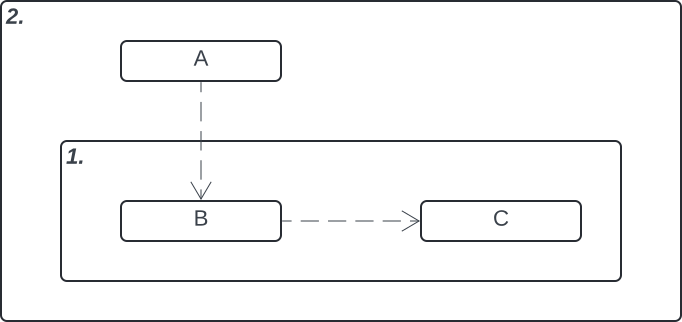
\includegraphics[scale=0.4]{part four/Testende Verfahren/img/bottomup}
    \caption{Beispiel für das Vorgehen bei der \textbf{Bottom-Up-Integration}. Im \textbf{Klassentest} wird für \textbf{B} ein Mock für \textbf{C} erstellt, für \textbf{A} ein Mock für \textbf {B}.\\
    Bei der Integration wird dann im ersten Schritt \textbf{B} und \textbf{C} integriert, im Erfolgsfall dann \textbf{A} und \textbf{B} und \textbf{C}. (Quelle: in Anlehnung an \cite[Abb. 5.5, 60]{Wed09c})}
    \label{fig:bottomup-cc}
\end{figure}